\documentclass[landscape]{slides}

\usepackage{amssymb}
\usepackage{alltt}
\usepackage{color}
\usepackage{code}
\usepackage{epsfig}
\usepackage{latexsym}

\newcommand{\cut}[1]{}

\newcommand{\appref}[1]{Appendix~\ref{#1}}
\newcommand{\secref}[1]{Section~\ref{#1}}
\newcommand{\tblref}[1]{Table~\ref{#1}}
\newcommand{\figref}[1]{Figure~\ref{#1}}
\newcommand{\listingref}[1]{Listing~\ref{#1}}
%\newcommand{\pref}[1]{{page~\pageref{#1}}}

\newcommand{\eg}{{\em e.g.}}
\newcommand{\cf}{{\em cf.}}
\newcommand{\ie}{{\em i.e.}}
\newcommand{\etc}{{\em etc.\/}}
\newcommand{\naive}{na\"{\i}ve}
\newcommand{\role}{r\^{o}le}
\newcommand{\forte}{{fort\'{e}\/}}
\newcommand{\appr}{\~{}}

\newcommand{\bftt}[1]{{\ttfamily\bfseries{}#1}}
\newcommand{\kw}[1]{\bftt {#1}}
\newcommand{\Pthen}{\kw{Pthen}}
\newcommand{\pads}{\textsc{pads}}
\newcommand{\padsl}{\textsc{padsl}}
\newcommand{\padst}{\textsc{pads/t}}
\newcommand{\datatype}{\textsc{PADS/T}}
%\newcommand{\datatype}{\textsc{DataType}}
\newcommand{\C}{\textsc{C}}
\newcommand{\perl}{\textsc{Perl}}
\newcommand{\ml}{\textsc{ml}}
\newcommand{\sml}{\textsc{sml}}
\newcommand{\smlnj}{\textsc{sml/nj}}
\newcommand{\java}{\textsc{java}}
\newcommand{\ddl}{\textsc{ddl}}
\newcommand{\xml}{\textsc{xml}}
\newcommand{\datascript}{\textsc{DataScript}}
\newcommand{\packettypes}{\textsc{PacketTypes}}
\newcommand{\erlang}{\textsc{Erlang}}

\newcommand{\Core}{Ad hoc}
\newcommand{\core}{ad hoc}
\newcommand{\pvalue}{\core{} value}
\newcommand{\ppat}{\core{} pattern}
\newcommand{\ptype}{\core{} type}

\newcommand{\padsc}{\textsc{pads}/\C{}}
\newcommand{\padsml}{\textsc{pads}/\ml{}}

\newcommand{\dibbler}{Sirius}
\newcommand{\ningaui}{Altair}
\newcommand{\darkstar}{Regulus}

\newcommand{\pdgood}{{\tt G}}
\newcommand{\pdbad}{{\tt B}}
\newcommand{\pdnest}{{\tt N}}
\newcommand{\pdsem}{{\tt S}}
\newcommand{\ptypes}{T}
\newcommand{\patreadpd}[2]{{\tt #1<<#2>>}}
\newcommand{\btm}{\cd{BOT}}


\newcommand{\lsem}{{[\![}}
\newcommand{\rsem}{{]\!]}}


\newcommand{\figHeight}[4]{\begin{figure}[tb]
	\centerline{
	            \epsfig{file=#1,height=#4}}
	\caption{#2}
	\label{#3}
	\end{figure}}

%% Environment for typesetting BNF grammars. Uses display math mode.
\newenvironment{bnf}
     {%% local command definitions:
        %% BNF definition symbol
      \def\->{\rightarrow}
%%      \def\::={{::=} &}
      \def\::={\bnfdef &}
      \def\|{\bnfalt}
      \newcommand{\name}[1]{\text{##1}}
        %% non-terminal
      \newcommand{\nont}[1]{{##1}}
      \newcommand{\meta}[1]{& ##1 &}
      \newcommand{\descr}[1]{& \text{// ##1}}
      \newcommand{\opt}[1]{ [##1] }
      \newcommand{\opnon}[1]{\opt{\nont{##1}}}
      \newcommand{\none}{\epsilon}
      \newcommand{\nwln}{\\ &&&}
      \newcommand{\nlalt}{\\ && \| &}
      \[\begin{array}{lrlll}
     }
     {\end{array}\]}

\newcommand{\mcd}[1]{\mathtt{#1}}
\newcommand{\ppair}[3]{#1{:}#2 \mathrel{**} #3}
\newcommand{\parray}[3]{#1\;\mcd{Parray}(#2,#3)}
\newcommand{\pset}[3]{\{#1{:}#2\,|\,#3\}}
\newcommand{\pstream}[1]{#1\;\mcd{stream}}
\newcommand{\precord}[1]{\{\{#1\}\}}


\definecolor{red}{rgb}{1,0.38,0.000}
\definecolor{darkgreen}{rgb}{0,0.8,0}

\newcommand{\eat}[1]{}

\newcommand{\blue}[1]{{\color{blue}#1}}
\newcommand{\red}[1]{{\color{red}#1}}
\newcommand{\green}[1]{{\color{green}#1}}
\newcommand{\darkgreen}[1]{{\color{darkgreen}#1}}
\newcommand{\yellow}[1]{{\color{yellow}#1}}
\newcommand{\black}[1]{{\color{black}#1}}
\newcommand{\white}[1]{{\color{white}#1}}
\newcommand{\grey}[1]{{\color{grey}#1}}
\newcommand{\mytt}[1]{{\tt #1}}

\newcommand{\ww}{\vspace{-1.5ex}}
\newcommand{\slidetitle}[1]{\red{\Large #1}\vspace{-1ex}}
\newcommand{\subtitle}[1]{\blue{#1}\ww}
\newcommand{\bluett}[1]{\texttt{\blue{#1}}}
\newcommand{\redtt}[1]{\texttt{\red{#1}}}
\newcommand{\bluerm}[1]{\textrm{\blue{#1}}}
\newcommand{\bx}[1]{\black{$#1$}}

\newcommand{\equals}{\blue{$=$}}
\newcommand{\subsumedby}{\blue{$\subseteq$}}
\newcommand{\notsubsumedby}{\blue{$\not\subseteq$}}

\newcommand{\lb}{\texttt{\symbol{123}}}
\newcommand{\rb}{\texttt{\symbol{125}}}
\newcommand{\br}[1]{\lb#1\rb}

\newcommand{\id}[1]{\texttt{#1}}
\newcommand{\bid}[1]{\id{\blue{#1}}}
\newcommand{\blid}[1]{\id{\black{#1}}}
\newcommand{\blit}[1]{\black{\emph{#1}}}

\newcommand{\eone}{$e_1$}
\newcommand{\etwo}{$e_2$}
\newcommand{\ethree}{$e_3$}
\newcommand{\vone}{$v_1$}
\newcommand{\vtwo}{$v_2$}
\newcommand{\evar}{$e$}
\newcommand{\vvar}{$v$}
\newcommand{\avar}{$a$}
\newcommand{\dvar}{$d$}

\newcommand{\var}[1]{\id{{\$}$#1$}}
\newcommand{\set}[1]{\{#1\}}
\newcommand{\att}[2]{\id{attribute $#1$ \br{ $#2$ }}}
\newcommand{\comatt}[2]{\id{attribute \br{ $#1$ } \br{ $#2$ }}}
\newcommand{\elt}[2]{\id{element $#1$ \br{ $#2$ }}}
\newcommand{\comelt}[2]{\id{element \br{ $#1$ } \br{ $#2$ }}}
\newcommand{\seq}{\mathbin{\id{,}}}
\newcommand{\choice}{\mathbin{\id{|}}}
\newcommand{\emp}{\id{()}}

\newcommand{\dsh}{\id{-}}
\newcommand{\str}{\id{*}}
\newcommand{\opt}{\id{?}}
\newcommand{\pls}{\id{+}}

\newcommand{\Primes}[1]{\mbox{P$'$($#1$)}}
\newcommand{\Prime}[1]{\mbox{P($#1$)}}
\newcommand{\Quant}[1]{\mbox{Q($#1$)}}

\newcommand{\at}{\id{@}}
\renewcommand{\slash}{\mathbin{\id{/}}}
\newcommand{\slashslash}{\mathbin{\id{//}}}
\newcommand{\brackets}[1]{\id{[$#1$]}}

\newcommand{\subst}[2]{\id{\{$\var{#1}$ := $#2$\}}}
\newcommand{\forloop}[3]{\id{for $\var{#1}$ in $#2$ return $#3$}}
\newcommand{\paren}[1]{\id{($#1$)}}

\newcommand{\Nextline}{\\ \\ \\}

\newenvironment{Slide}[1]{\begin{slide}\slidetitle{#1}}{\vfill\end{slide}}

\newenvironment{TitleSlide}[2]{\begin{slide}
\begin{center}\LARGE\color{red}#1\large\color{blue}#2}{\end{center}
\end{slide}}

\newcounter{partctr}
\renewcommand{\thepartctr}{\Roman{partctr}}
\newcounter{subpartctr}[partctr]
\renewcommand{\thesubpartctr}{\Roman{partctr}.\arabic{subpartctr}}

\newcommand{\partslide}[1]{
 \begin{slide}
 \begin{center}\Large\color{blue}
 \refstepcounter{partctr}
 Part \thepartctr\\[2ex]\LARGE\color{red}
 #1
 \end{center}
 \end{slide}
}

\newcommand{\prologslide}[1]{
 \begin{slide}
 \begin{center}\Large\color{blue}
 Prolog\\[2ex]\LARGE\color{red}
 #1
 \end{center}
 \end{slide}
}

\newcommand{\preludeslide}[1]{
 \begin{slide}
 \begin{center}\Large\color{blue}
 Prelude\\[2ex]\LARGE\color{red}
 #1
 \end{center}
 \end{slide}
}

\newcommand{\interludeslide}[1]{
 \begin{slide}
 \begin{center}\Large\color{blue}
 Interlude\\[2ex]\LARGE\color{red}
 #1
 \end{center}
 \end{slide}
}

\newcommand{\epilogslide}[1]{
 \begin{slide}
 \begin{center}\Large\color{blue}
 Epilog\\[2ex]\LARGE\color{red}
 #1
 \end{center}
 \end{slide}
}

\newcommand{\subpartslide}[1]{
 \begin{slide}
 \begin{center}\Large\color{blue}
 \refstepcounter{subpartctr}
 Part \thesubpartctr\\[2ex]\LARGE\color{red}
 #1
 \end{center}
 \end{slide}
}

\newcommand{\quoteslide}[2]{
 \begin{slide}
 \begin{quote}
 \blue{#1}
 \begin{flushright}
 \red{--- #2}
 \end{flushright}
 \end{quote}
 \end{slide}
}

\newenvironment{tightitemize}{
  \begin{list}{$\bullet$}{
    \setlength{\topsep}{0ex}
    \setlength{\itemsep}{1ex}
    \setlength{\parsep}{0ex}
    \setlength{\partopsep}{0ex}
  }
}{
  \end{list}
}

\newenvironment{tighteritemize}{
  \begin{list}{$\bullet$}{
    \setlength{\topsep}{0ex}
    \setlength{\itemsep}{0ex}
    \setlength{\parsep}{0ex}
    \setlength{\partopsep}{0ex}
  }
}{
  \end{list}
}

\newcommand{\bluetriangle}[0]{{\blue{$\blacktriangleright$}}}
\newcommand{\whitetriangle}[0]{{\white{$\blacktriangleright$}}}
\newcommand{\greentriangle}[0]{{\green{$\blacktriangleright$}}}
\newcommand{\redtriangle}[0]{{\red{$\blacktriangleright$}}}

\newcommand{\lbluetriangle}[0]{{\blue{$\blacktriangleleft$}}}
\newcommand{\lgreentriangle}[0]{{\green{$\blacktriangleleft$}}}
\newcommand{\lredtriangle}[0]{{\red{$\blacktriangleleft$}}}

\newcommand{\vl}{\vspace*{0.5cm}}
\newcommand{\vv}{\vspace*{1cm}}
\newcommand{\hh}{\hspace*{0.5cm}}
\newcommand{\hhh}{\hspace*{0.8cm}}

\newcommand{\bb}{\redtriangle\ }
\newcommand{\dbb}{\redtriangle\redtriangle\ }
\newcommand{\bbb}{\hhh\bluetriangle\ }
\newcommand{\bbw}{\hhh\whitetriangle\ }
\newcommand{\bbbb}{\hhh\hhh\greentriangle\ }

\newcommand{\lbb}{\lredtriangle}
\newcommand{\ldbb}{\ \lredtriangle\lredtriangle}

\newcommand{\redbr}[1]{\red{\lb}#1\red{\rb}}
\newcommand{\arrow}{\Rightarrow}

\sloppy \setlength{\topmargin}{0in} \addtolength{\topmargin}{-1.0in}
\addtolength{\textheight}{1.5in}



\newcommand{\scream}[1]{\textbf{#1}}

\newcommand{\notes}[1]{{\tiny #1}}
%\newcommand{\notes}[1]{}

\newcounter{chap}
\stepcounter{chap}

%%%%%%%%%%%%%%%%%%%%%%%%%%%%%%%%%%%%%%%%%%%%%%%%%%%%%%%%%%%%%%%%%%%%%%%%
\begin{document}
%%%%%%%%%%%%%%%%%%%%%%%%%%%%%%%%%%%%%%%%%%%%%%%%%%%%%%%%%%%%%%%%%%%%%%%%

% Title slide
\begin{slide}
\begin{center}\LARGE\color{blue}
The PADS-Galax Project: \\
Enabling XQuery over  Ad-hoc Data Sources

Yitzhak Mandelbaum
\end{center}
\end{slide}

\begin{Slide}{Existing Technologies}
  
  \vspace*{1cm}
  \bb What is PADS?\\
  \bbb Declarative data-stream description language\\
  \bbb Syntax \& semantics of \blue{semi-structured}, legacy data sources \\
  \bbb Compiler generates data-parsing library from description\\
  \bbb Library detects \& recovers from non-fatal errors in data

  \bb What is Galax?\\
  \bbb Complete, extensible implementation of XQuery 1.0 

  \bb What is XQuery?\\
  \bbb Functional, strongly typed XML query language \\
  \bbb Well-suited to querying \blue{semi-structured} sources

\end{Slide}

\begin{Slide}{Describing HTTP Common Log Format}

  \bb Data

{\small
\begin{alltt}
\blue{207.136.97.49 - - [15/Oct/1997:18:46:51 -0700] "GET /tk/p.txt HTTP/1.0" 200 30}
\end{alltt}
}
  \bb PADS Description

{\small
\begin{alltt}
\kw{Pstruct} http_request_t \{
  '\verb|\"|'; http_method_t    meth;           /- Method used during request
  ' ';  Pa_string(:' ':) req_uri;        /- Requested uri.
  ' ';  http_v_t         version : checkVersion(version, meth);
                                         /- HTTP version number of request 
  '\verb|\"|';
\};
\end{alltt}
}

\end{Slide}

\begin{Slide}{Viewing \& Querying HTTP CLF}

  \bb Virtual XML Data
{\tiny
\begin{alltt}
\blue{<http-clf>
  <host>207.136.97.49</host>
  <remoteID>-</remoteID>
  <auth>-</auth>
  <mydate>15/Oct/1997:18:46:51 -0700</mydate>
  <request><meth>GET</meth><req_uri>/tk/p.txt</req_uri><version>HTTP/1.0 ...
  <response>200</response>
  <contentLength>30</contentLength>
<http-clf>}
\end{alltt}
}

\bb Selection \& projection using XQuery\\
\bbb Return hosts of CLF records with content length greater than 2K

{\small
\begin{alltt}
\blue{\$pads-doc/http-clf[contentLength > 2048]/host}
\end{alltt}}

\bb Vet errors in data using XQuery \\
\bbb Return locations of records with error in content-length field

{\small
\begin{alltt}
\blue{\$pads-doc/http-clf[contentLength/@pads:errCode]/@pads:loc}
\end{alltt}}
\end{Slide}

\begin{Slide}{Technical Challenges}

  \bb Define mapping from PADS description to XML Schema 

  \bb Materialize PADS data as virtual XML \\
  \bbb Galax has extensible data model \\
  \bbb Implement Galax's abstract data model on top of PADS 

  \bb Memory management of PADS records \\
  \bbb Data exceeding memory limits requires clever MM\\
  \bbb PADS program typically reads records sequentially \\
  \bbb Galax may not access records sequentially 

  \bb User-friendly interface\\
  \bbb Describe PADS data, compile library, write \& execute queries

\end{Slide}

\begin{Slide}{Technical Challenges \& Solutions}

  \bb Define mapping from PADS description to XML Schema \\
  \bbb Canonical mapping defined Summer 2003

  \bb Materialize PADS data as virtual XML \\
  \bbb Started Summer 2003 but incomplete \\
  \bbb Align with current Galax Data Model

  \bb Memory management of PADS records \\
  \bbb Focus in Summer 2004

  \bb User-friendly interface\\
  \bbb Room for improvement

\end{Slide}

\begin{Slide}{PADS-Galax Architecture} 

  \vspace*{1cm}
  \centerline{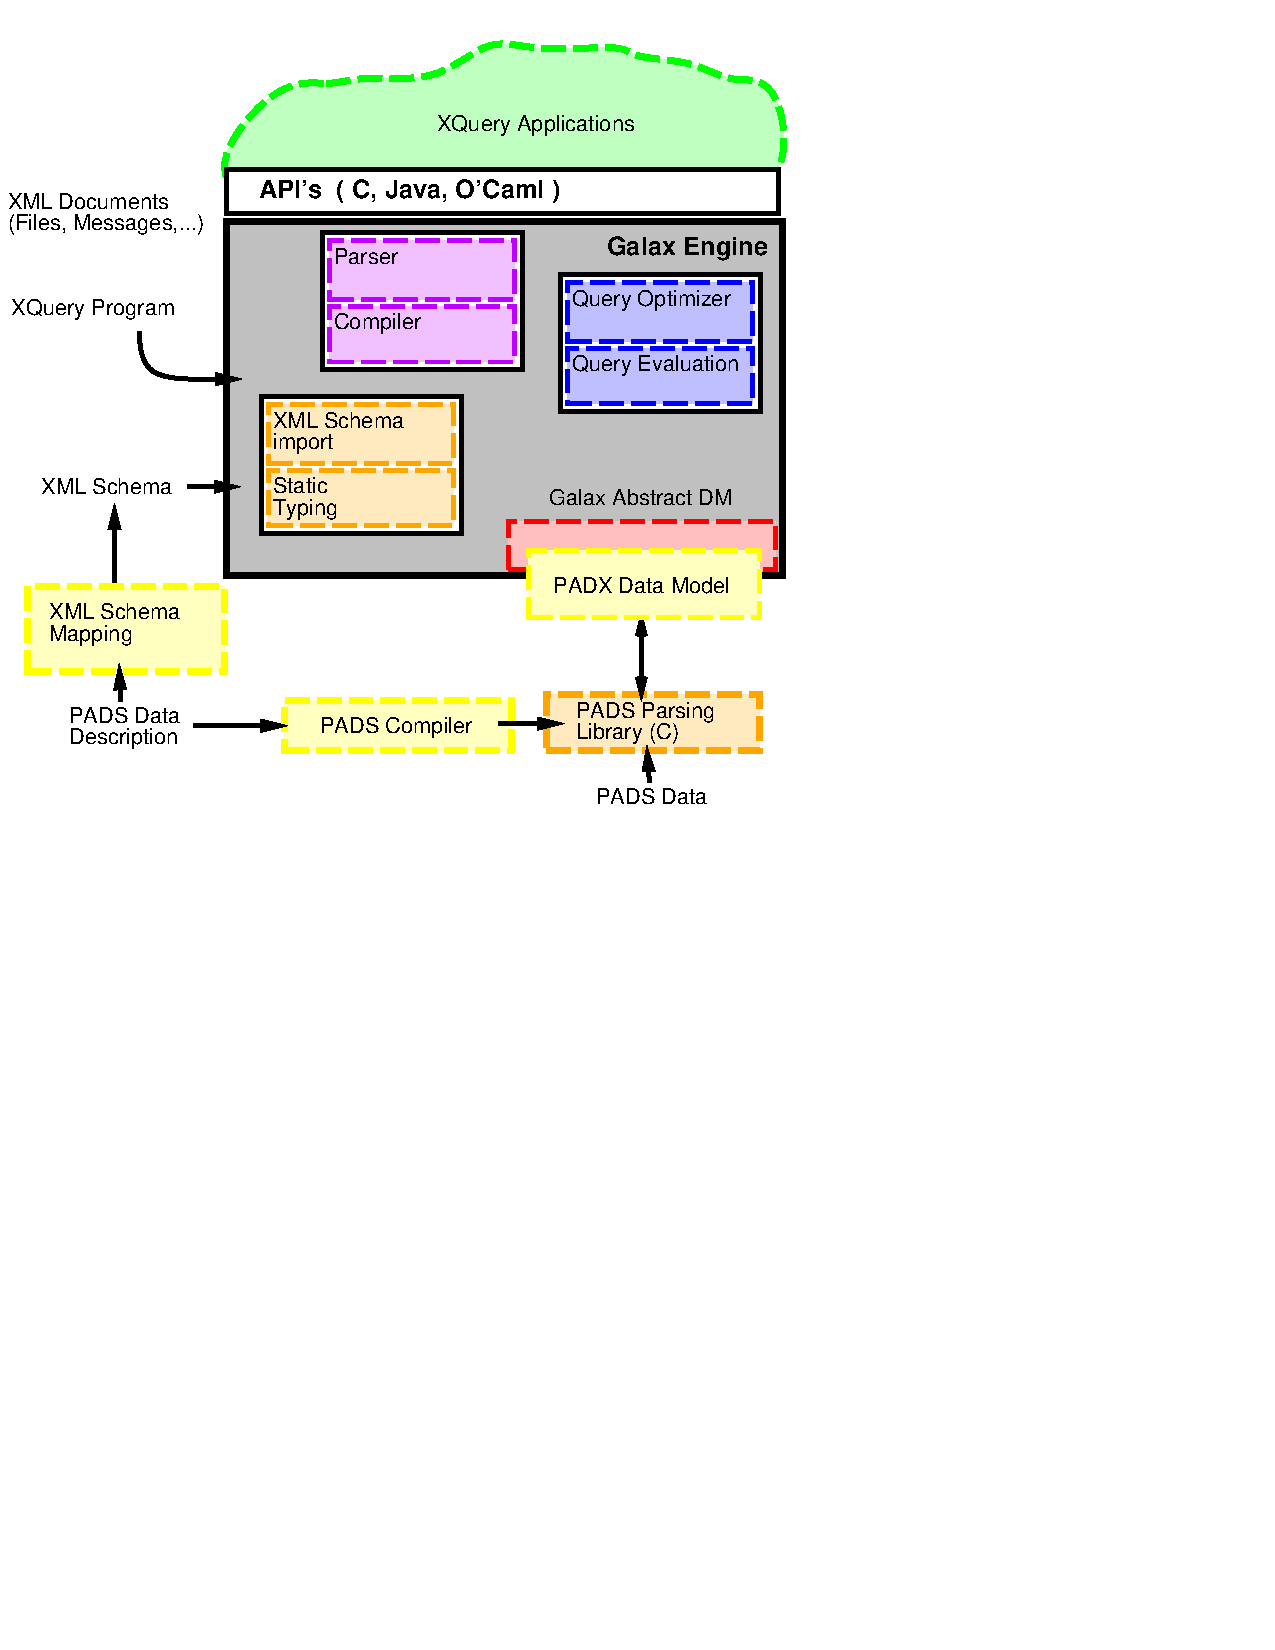
\psfig{file=pads-galax-overview-yitzhak.pdf}}
\end{Slide}

\begin{Slide}{Abstract Node Interface}

  \vspace*{1cm}
\bb Fragment of Galax's abstract XML node interface\\
\bbb Full navigation of XML tree\\
\bbb Access to atomic values

{\small
\begin{alltt}
  method virtual \blue{node_name}    : unit -> atomicQName option

  method virtual \blue{typed_value}  : unit -> atomicValue cursor

  method virtual \blue{parent}       : unit -> node option
  method virtual \blue{children}     : unit -> \green{node cursor}

  method virtual \blue{docorder}  : unit -> Nodeid.docorder
\end{alltt}}

\bb Cursor : lazy iterator access to node sequence\\
\bb Node identity \& document order : canonical order 

\end{Slide}

\begin{Slide}{Accessing Record Sequences}

  \bb Access to record (node) sequence \\
  \bbb Read all items in sequence \\
  \bbb Produce items on demand

  \bb Each record field materialized strictly as needed

  \bb Solution: \\
  \bbb Choose record as read granularity \\
  \bbb Read record on demand \\
  \bbb Maintain meta-data for fast re-retrieval

%   \bb paging, with element as page granularity
%   \bb tmap, page-table for elements 
%   \bb (for finer granularity, group
%     elements into fixed-size arrays)
\end{Slide}

\begin{Slide}{smart arrays - weak references}

  \bb data references can't be trusted
  \bb challenge: irregular structure of elements. 

    \bbb finding element is not enough.
    \bbb store pointers in page members.
    \bbb guard with gen.
    \bbb gen invalidated when elt. evicted.

\end{Slide}

\begin{Slide}{Rereading an element}

  \bb Pads elements are read in full.
  \bb Designed incremental read function.
  \bb non trivial due to the complexity of the array termination semantics.
  \bb reread can't modify parse-descriptor.

\end{Slide}

\begin{Slide}{Project Status}

\bb Integration effort successful 

\bb More thorough regression testing

\bb Demonstrate to potential users

\bb Research problems\\
\bbb Extending Galax's data model to leverage streams access\\
\bbb More efficient meta-data structures in PADS 

\end{Slide}

% \begin{Slide}{Demo slide}
%   , showing commands needed to get up and running.
% \end{Slide}


% \begin{Slide}{Project Challenges}
%   \bb learning all the pieces
%   \bb dividing between macros and compiler
%   \bb dividing between type-specific code and polymorphic macros.
% \end{Slide}

\begin{Slide}{thanks to Kathleen, Bob, and Mary!}
\end{Slide}

%%%%%%%%%%%%%%%%%%%%%%%%%%%%%%%%%%%%%%%%%%%%%%%%%%%%%%%%%%%%%%%%%%%%%%%%
\end{document}
%%%%%%%%%%%%%%%%%%%%%%%%%%%%%%%%%%%%%%%%%%%%%%%%%%%%%%%%%%%%%%%%%%%%%%%%

